\begin{figure}[ht]
\centering
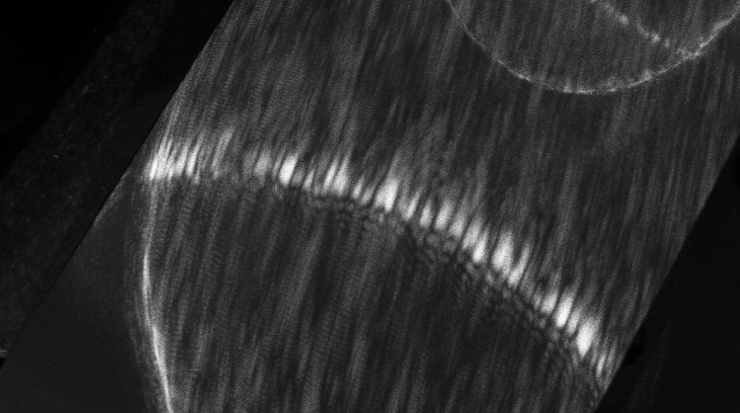
\includegraphics[keepaspectratio,width=15cm]{speckle/figures/Ag_LaSFN9_cone_lens11_cam-8899.jpg}
\caption{A portion of the cone speckle, distorted by a lens and projected onto a piece of paper.}
\label{fig:examplespeckle}
\end{figure}
\section{Introduction}

Under most circumstances, light in the cone is not spatially homogeneous but
exhibits distinctive intensity fluctuations known as \textit{speckle}, which
arise from the interference of multiple coherent waves with statistically
random amplitudes and phases.  In optics, speckle is closely related to the
mesoscopic phenomena of universal conductance
fluctuations~\cite{lee1985universal} and it likewise exhibits many of the same
physical phenomena such as coherent
backscattering~\cite{akkermans1986coherent} and the memory
effect~\cite{freund1988memory}.

Speckle is also known to host a wealth of interesting
properties~\cite{goodman1975statistical}~\cite{freund19981001}, particularly
in the multiple scattering regime~\cite{feng1986sensitivity} where it has been
shown to be extraordinarily sensitive to both the position and
motion~\cite{berkovits1994correlations} of its underlying scatterers.  Indeed,
in this way speckle may be seen as a unique
fingerprint~\cite{ravikanth2001physical} of the underlying scattering
microstructure.  Such principles have already been exploited in a diverse set
of applications such as diffusing wave spectroscopy~\cite{pine1988diffusing}
and dynamic light scattering~\cite{berne2000dynamic} in the time domain.
Furthermore, speckle has been shown to be sensitive to the sub-wavelength
motions~\cite{berkovits1991sensitivity} or
inclusions~\cite{berkovits1990theory} of even single scatterers.

As there is no prior work related to cone speckle, the present chapter begins
with the mathematical and statistical properties of generalized speckle
fields, and how well the speckle in the cone can be described by them.  In
particular, two important characteristic properties of speckle, size
and contrast, will be measured and compared with the theory.  Any specific
influence regarding dynamic changes in the underlying scattering
microstructure are reserved for \Chapter{ch:scatteringmicro}.

\subsection{Objective Speckles}
Speckle produced by the \gls{spp} scattering geometry in
\Figure{fig:experimentalsetup}, when measured by an imaging sensor in the far
field (Fraunhoffer regime), is known as \textit{objective speckle}.  Features
of objective speckle are typically not applicable to speckle obtained in e.g.\
the near field regime.  Most pertinent, the mean speckle size is approximately
given by $\lambda z/d$, where $\lambda$ is the wavelength, $z$ is the
propagation distance, and $d$ is the transverse dimension of the scattering
spot\cite{dainty1975laser}.
